\documentclass{beamer}
\usetheme{Madrid}
\setbeamertemplate{bibliography item}{\insertbiblabel}

\usepackage[main=english,czech]{babel}
\usepackage[utf8]{inputenc}
\usepackage{url}
\usepackage{caption}

\captionsetup[figure]{font=footnotesize}

%\usepackage{biblatex}
%\addbibresource{references.bib}

\AtBeginSection[]
{
	\begin{frame}<beamer>[noframenumbering]
		\frametitle{Outline}
		\tableofcontents[currentsection]
	\end{frame}
}

\title[Atypic TPC track simul. \& reconstruction]{Simulation and reconstruction of charged particle trajectories in an atypic time projection chamber}
%\subtitle{Subtitle}
\author[M.~Vavřík]{\foreignlanguage{czech}{Martin Vavřík}\vspace{0.5cm}\\martin.vavrik@cvut.cz\\IEAP CTU PRAGUE\\}
\logo{
\includegraphics[width=0.08\textwidth]{../images/logo}}
\date{March 7, 2023}

\begin{document}
	
	\begin{frame}
		\titlepage
	\end{frame}
	
	\begin{frame}
		\frametitle{Outline}
		\tableofcontents
	\end{frame}
	
	\section{Motivation}
	\begin{frame}
		\frametitle{Motivation}
		\begin{itemize}
			\item Measurement of anomalies in angular correlation of electron and positron internally produced in excited $ {}^8\text{Be} $ and $ {}^4\text{He} $
			\item For energy reconstruction, tracks in the time projection chamber (TPC) will be used
				\begin{itemize}
					\item Atypical TPC (magnetic field is perpendicular instead of parallel to electric)
					\item This interferes with the direction of the drift of electrons
					\item Energy can be determined using curvature of the track in the inhomogeneous magnetic field
					\item Magnetic field data from simulation is used
				\end{itemize}
		\end{itemize}
	\end{frame}

	\begin{frame}
		\frametitle{X17 detector}
		\begin{columns}
			\column{0.5 \textwidth}
				\begin{figure}
					\centering
					$ $\newline
					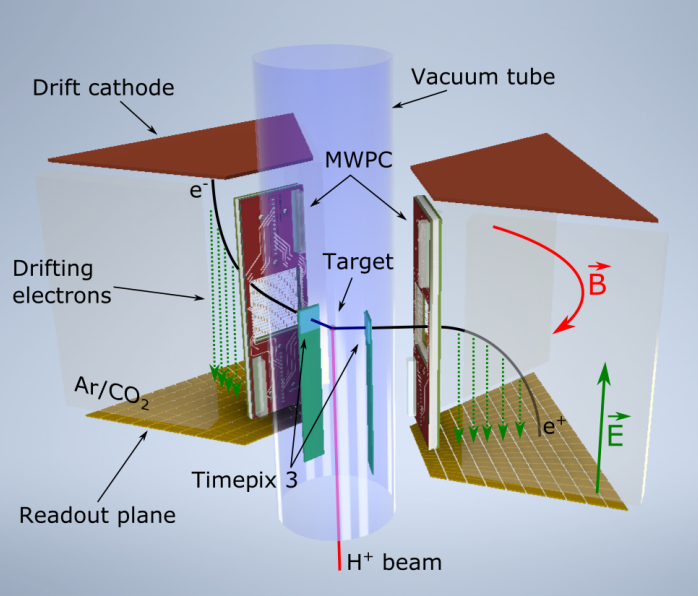
\includegraphics[width=0.81\linewidth]{../images/diagram.png}\newline
					\caption{A diagram of the X17 detector. You can see two out of the six TPC chambers.\cite{poster}}
					\label{fig:dia}
				\end{figure}
			\column{0.5 \textwidth}
				\begin{figure}
					\centering
					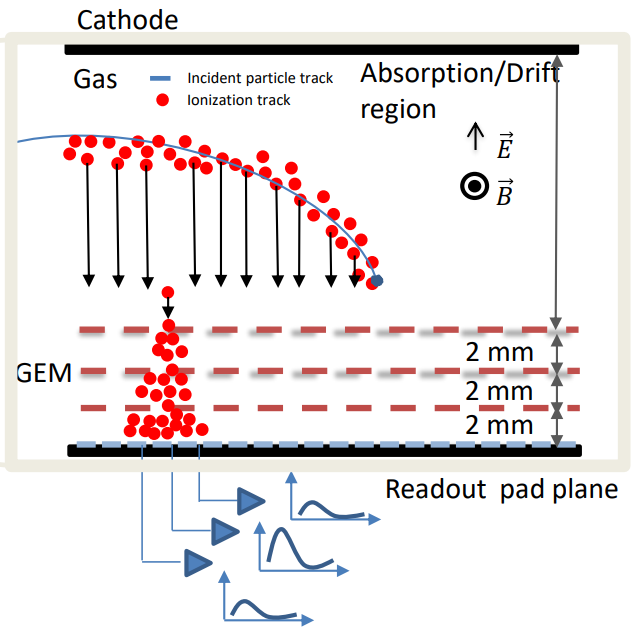
\includegraphics[width=0.82\linewidth]{../images/diagram2.png}
					\caption{Working principle of TPC with triple gas electron multiplier (GEM) readout.\cite{poster}}
					\label{fig:dia2}
				\end{figure}
		\end{columns}
	\end{frame}
	
	\section{Track simulation}
	\begin{frame}
		\frametitle{Track simulation}
		\begin{itemize}
			\item We use Garfield++ for track simulation
			\begin{itemize}
				\item Primary relativistic particle simulated using Heed program~\cite{heed}
				\item Secondary ionization electrons can be simulated using Monte Carlo (gas table calculation necessary)
				\item Alternative approach is microscopic tracking (uses equation of motion)
				\begin{itemize}\item A bit slower, more precise especially for small structures.  \end{itemize}
			\end{itemize}
			\item Currently we simulate only one track at a time for testing purposes
		\end{itemize}
	\end{frame}
	
	\begin{frame}
		\frametitle{Simulated track example (microscopic tracking)}		
		\begin{columns}
			\column{0.33\textwidth}
			\begin{figure}
				\centering
				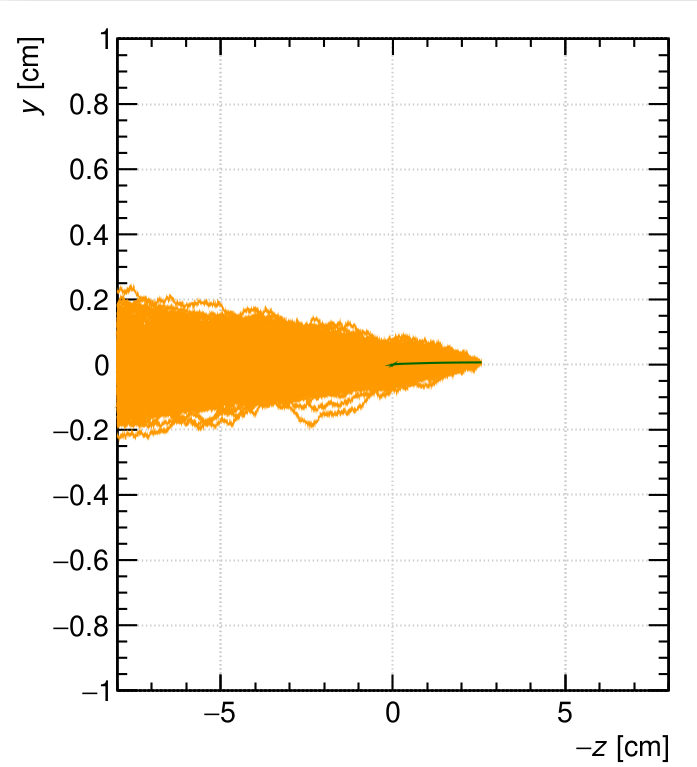
\includegraphics[width = 0.95 \linewidth]{../images/track1.png}
				\caption{Diffusion front view}
			\end{figure}
			\column{0.33\textwidth}
			\begin{figure}
				\centering
				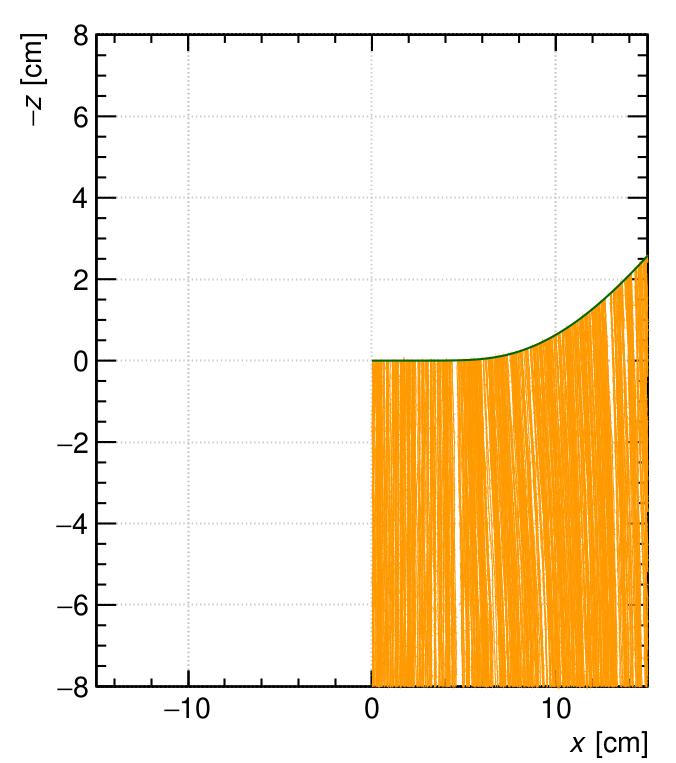
\includegraphics[width = 0.95 \linewidth]{../images/track2.png}
				\caption{Electron drift}
			\end{figure}
			\column{0.33\textwidth}
			\begin{figure}
				\centering
				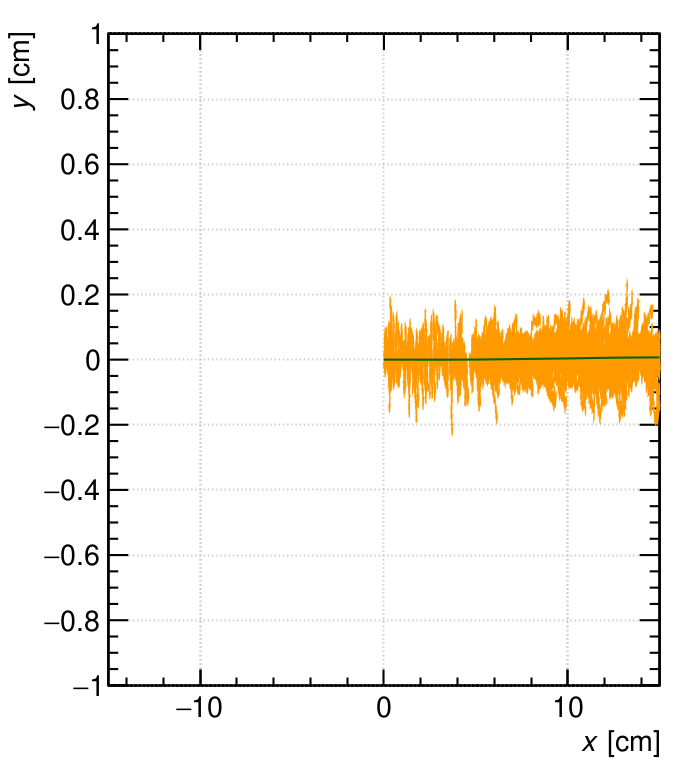
\includegraphics[width = 0.95 \linewidth]{../images/track3.png}
				\caption{Diffusion top view}
			\end{figure}
		\end{columns}
	\end{frame}

	\begin{frame}
		\frametitle{Ionization electrons map simulation}
		\begin{itemize}
			\item In the experimental setup TPC only detects secondary ionization electrons (after multiplication on triple GEM)
			\item These electrons drift at constant velocity towards the readout plane
			\item We can use simulation of evenly spaced electrons for reconstruction (time consuming -- run on MetaCentrum)
		\end{itemize}
		\begin{figure}
			\centering
			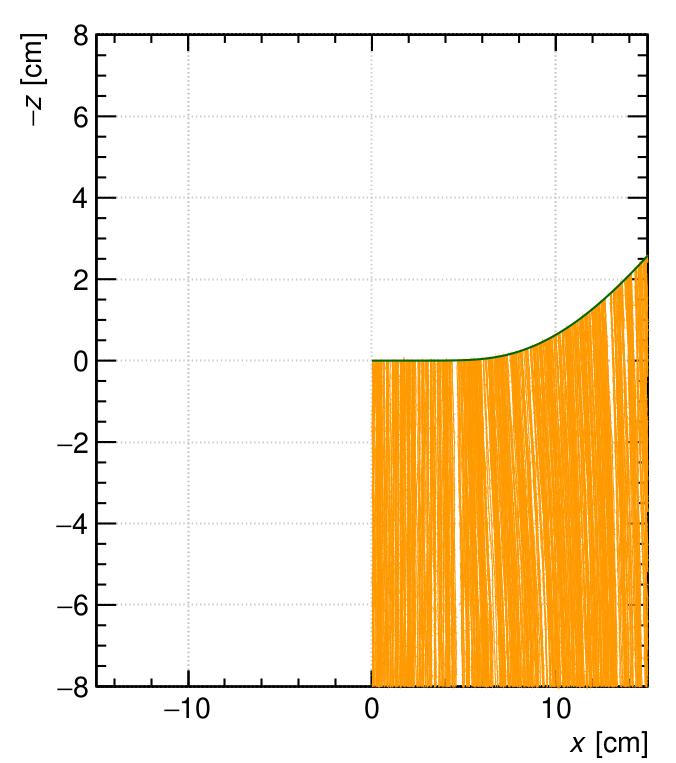
\includegraphics[width = 0.3 \linewidth]{../images/track2.png}
			\caption{Electron drift}
		\end{figure}
	\end{frame}

	\begin{frame}
		\frametitle{Ionization electron map simulation}
		\begin{itemize}
			\item As a result we get an approximation of a mapping from initial coordinates of the electrons $(x,y,z)$ to the readout coordinates $(x',y',t)$
			\item By interpolating we can get the inverse map
			\item We can use the inverse map to finally create mapping from our discrete readout values (channel number, time) to voxels of the primary track
		\end{itemize}
		\begin{figure}
			\centering
			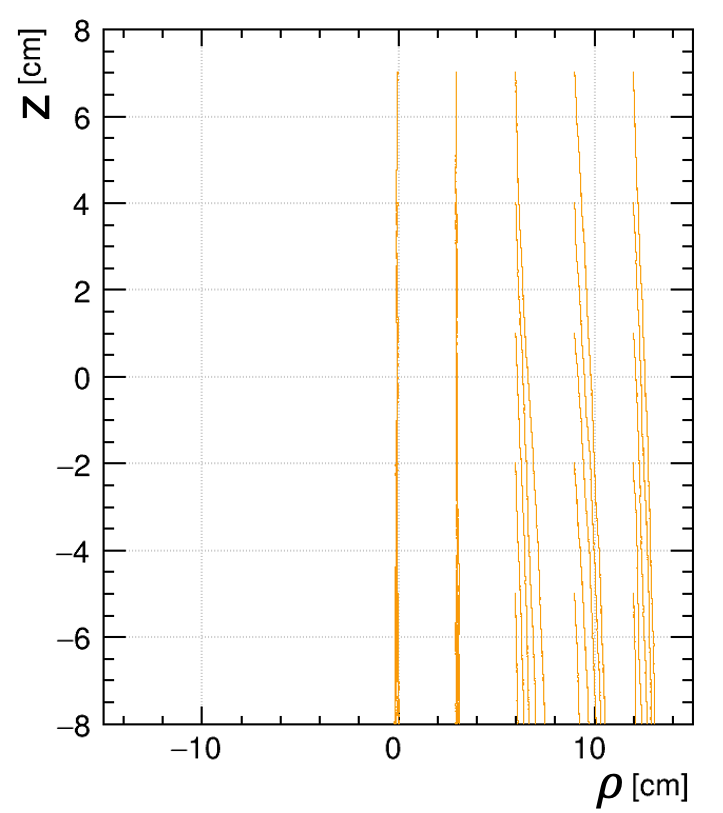
\includegraphics[height=0.4\textheight]{../images/map_lines.png}
			\caption{Partial simulation of the map}
		\end{figure}
	\end{frame}
	\begin{frame}
		\frametitle{Ionization electron map simulation}
		\begin{figure}
			\centering
			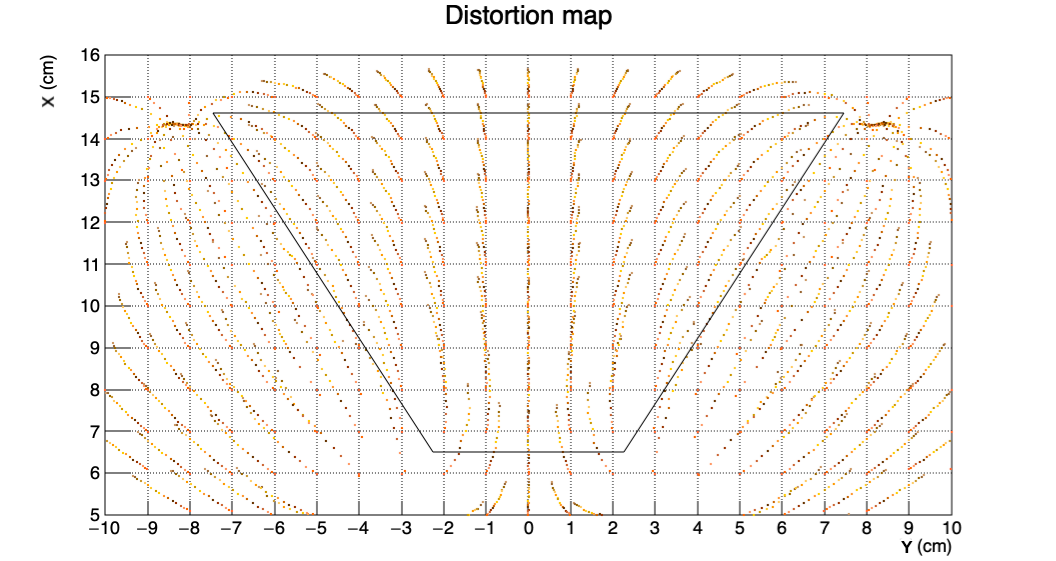
\includegraphics[height=0.6\textheight]{../images/map_dist.png}
			\caption{$x$ and $y$ coordinate distortion at different $z$ values (Credit: Hugo Natal da Luz).}
		\end{figure}
	\end{frame}
	\begin{frame}
		\frametitle{Ionization electron map simulation}
		\begin{figure}
			\centering
			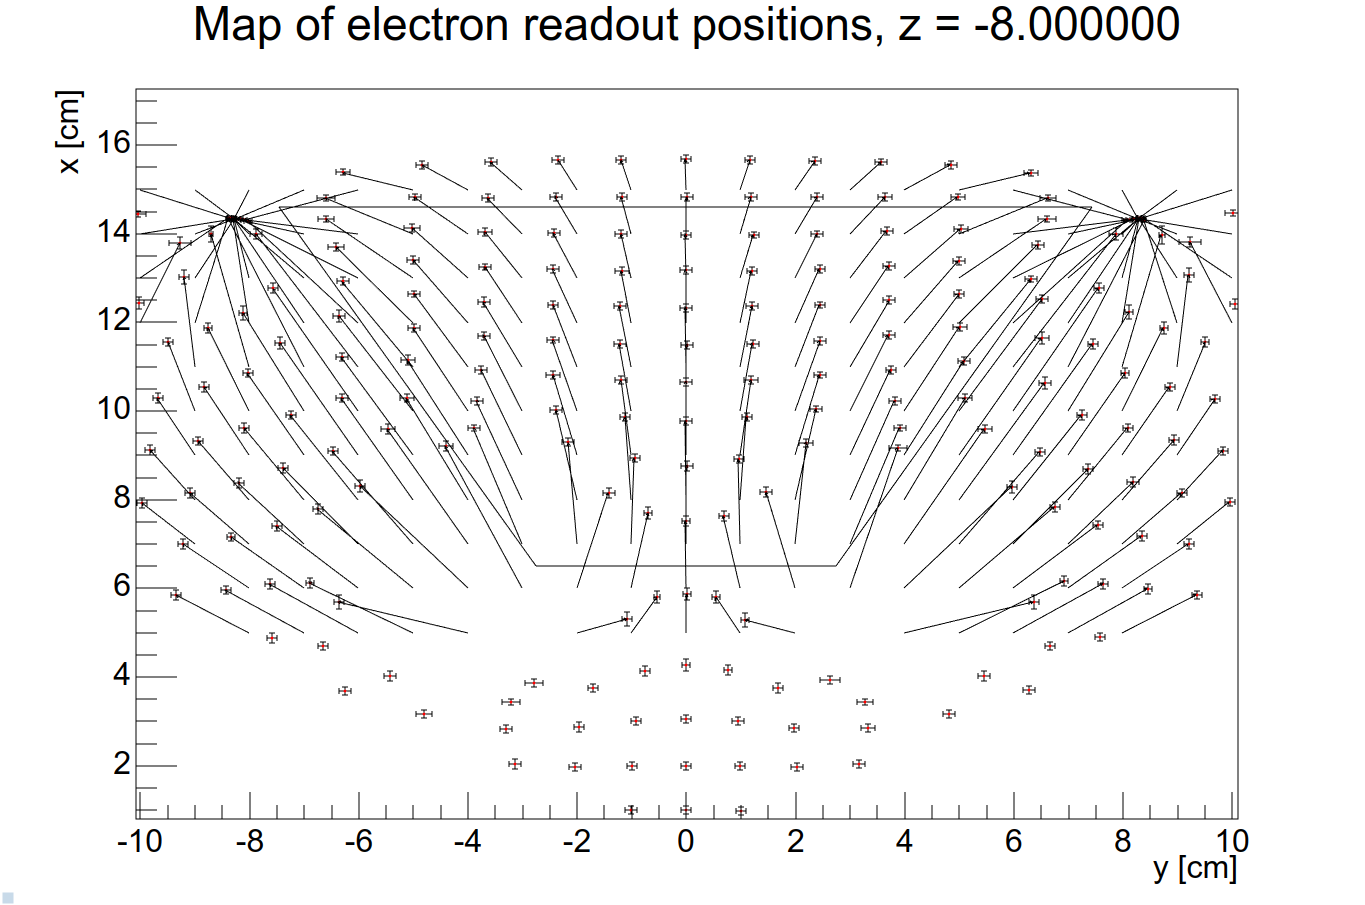
\includegraphics[height=0.65\textheight]{../images/map_dist2.png}
			\caption{$x$ and $y$ coordinate distortion for maximal initial distance from readout}
		\end{figure}
	\end{frame}
	\begin{frame}
		\frametitle{Ionization electron map simulation}
		\begin{figure}
			\centering
			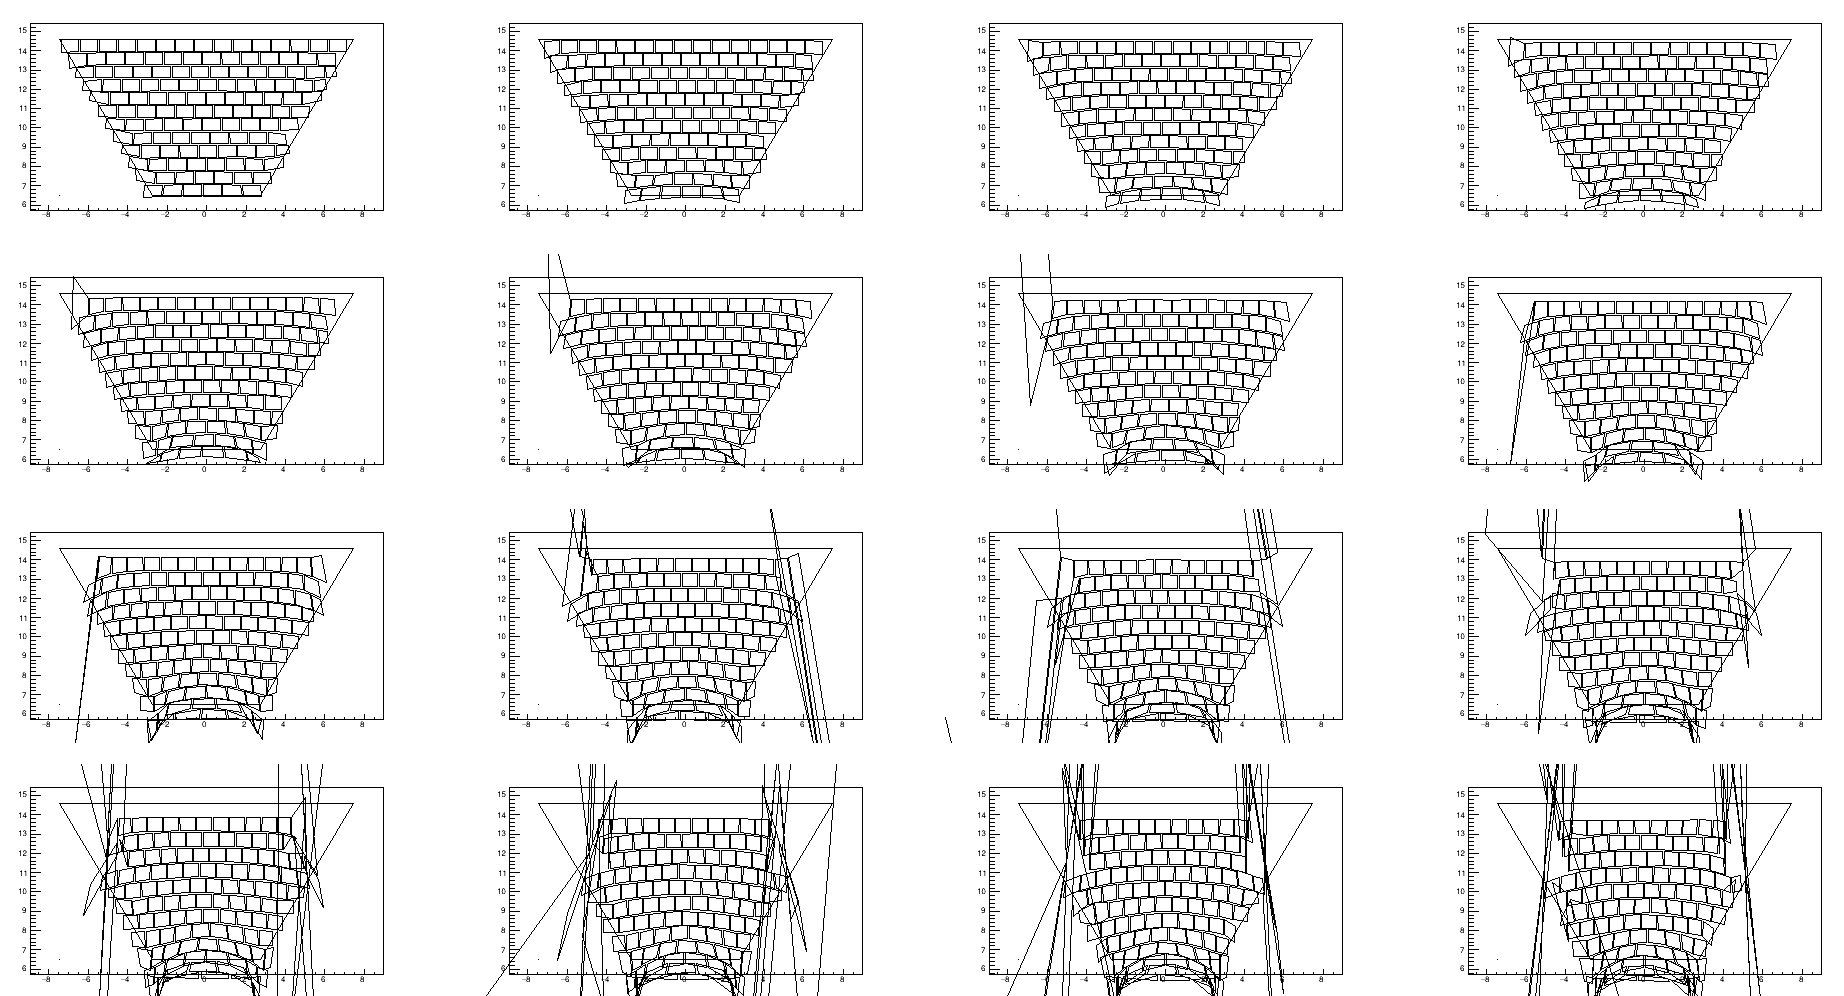
\includegraphics[height=0.68\textheight]{../images/pads_dist.png}
			\caption{Pad voxel boundaries for different times (picture of first attempt).}
		\end{figure}
	\end{frame}


	\section{Track reconstruction}
	\begin{frame}
		\frametitle{Track reconstruction}
		\begin{itemize}
			\item So far only preliminary attempts using the inverse map have been made (not accounting for readout pads)
		\end{itemize}
		\begin{figure}
			\centering
			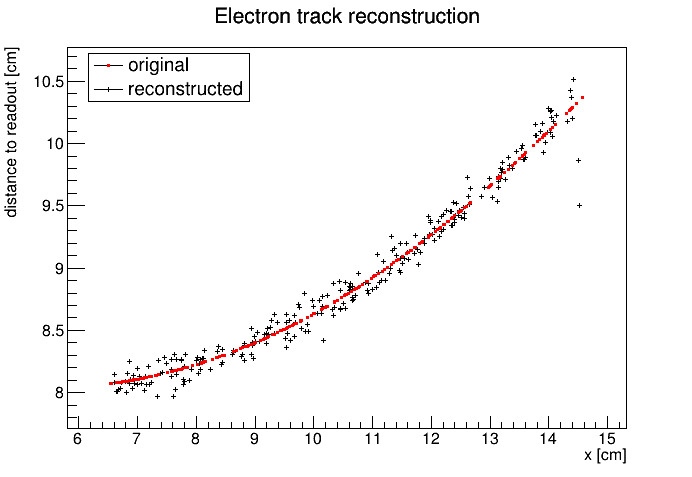
\includegraphics[width=0.6\textwidth]{../images/reco_track.png}
			\caption{Original and reconstructed interaction points on the simulated track}
		\end{figure}
	\end{frame}

	\section{Energy reconstruction}
	\begin{frame}
		\frametitle{Energy reconstruction}
		\begin{itemize}
			\item So far only preliminary attempts
			\item Best result for track fit with smoothly attached circular arc with straight lines (expected in homogeneous field)
			\item This or similar approach might be used as initial guess for the actual reconstruction
		\end{itemize}
		\begin{figure}
			\centering
			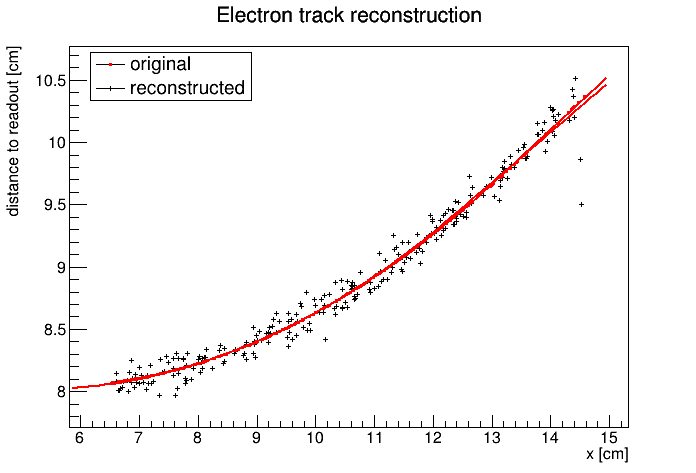
\includegraphics[width=0.5\textwidth]{../images/reco_e.png}
			\caption{8 MeV simulated electron energy reconstruction from both original and reconstructed interaction points. Results are 8.27 and 7.93 MeV.}
		\end{figure}		
	\end{frame}
	
	
	\section{Summary \& Future}	
	\begin{frame}
		\frametitle{Summary}
		\begin{itemize}
			\item Several tracks have been simulated for testing purposes
			\item The map of secondary electron positions and drift times has been generated
			\item The map has been tested by preliminary track reconstruction
			\item First attempts for energy reconstruction that might be useful as initial guesses
		\end{itemize}
	\end{frame}
	\begin{frame}
		\frametitle{Future}
		\begin{itemize}
			\item Account for GEM in simulation, charge distribution between pads
			\item Account for pads and discrete time in track reconstruction (irregular voxels)
			\item Use Runge-Kutta integration for energy reconstruction
				\begin{itemize}
					\item Reasonable initial guess of track parameters
					\item Likelihood optimization (voxels)
				\end{itemize}
			\item Simulate many tracks with random initial parameters to test the reconstruction
		\end{itemize}
	\end{frame}
	
	{
		%\usebackgroundtemplate{\includegraphics[width=\paperwidth,height=\paperheight]{../images/DSC_5602.jpg}}%
		\begin{frame}[noframenumbering]{}
			\begin{center}
				\Huge Thank you for your attention.
			\end{center}
		\end{frame}
	}
	
	%\section{References}
	\begin{frame}[allowframebreaks,noframenumbering]
		\frametitle{References}
		%\printbibliography
		\bibliography{../references}
		\bibliographystyle{unsrt}
	\end{frame}
	
\end{document}